\chapter {Model Editor}
\label{chap7}
\thispagestyle{empty}

Spice based simulators include a feature which allows accurate modeling
of semiconductor devices such as diodes, transistors etc. eSim Model
Editor provides a facility to define a new model for devices such as
\textit{diodes, MOSFET, BJT, JFET, IGBT, Magnetic core} etc. Model Editor in
eSim lets the user enter the values of parameters depending on the type of 
device for which a model is required. The parameter values can be
obtained from the data-sheet of the device. A newly created model can be
exported to the model library and one can import it for different
projects, whenever required. Model Editor also provides a facility to
edit existing models. The GUI of the model editor is as shown in \figref{modeleditor}

\begin{figure}
\centering
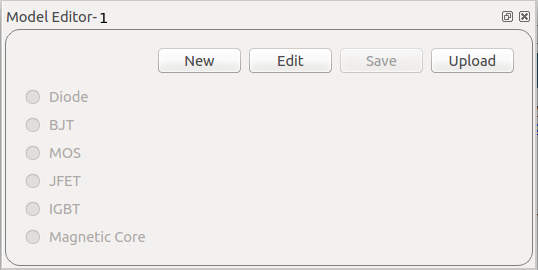
\includegraphics[width =\lgfig]{modeleditor_new.png}
\caption{Model Editor}
\label{modeleditor}
\end{figure} 

\section{Creating New Model Library }

eSim lets us create new model libraries based on the template model libraries.
On selecting {\tt New} button the window is popped as shown in \figref{modeleditor_new}. The name has to be unique otherwise the error message appears on the window.

\begin{figure}
\centering
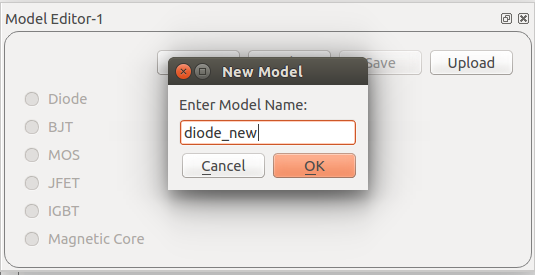
\includegraphics[width =\lgfig]{modeleditor.png}
\caption{Creating New Model Library}
\label{modeleditor_new}
\end{figure}
After the OK button is pressed the type of model library to be created is chosen by selecting one of the types on the left hand side i.e.{ \tt Diode, BJT, MOS, JFET, IGBT, Magnetic Core}. The template model library opens up in a tabular form as shown in \figref{modelnew}
\begin{figure}
\centering
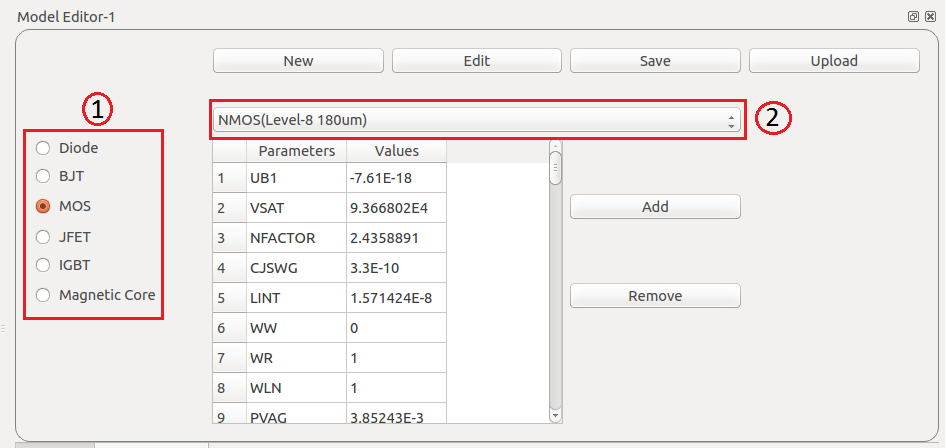
\includegraphics[width =\lgfig]{modelnew.png}
\caption{Choosing the Template Model Library }
\label{modelnew}
\end{figure}

\pagebreak

New parameters can be added or current parameters can be removed using {\tt ADD} and {\tt REMOVE} buttons. Also the values of parameters can be changed in the table. Adding and removing the parameters in library files is shown in the \figref{modeladd} and \figref{modelremove}

\begin{figure}
\centering
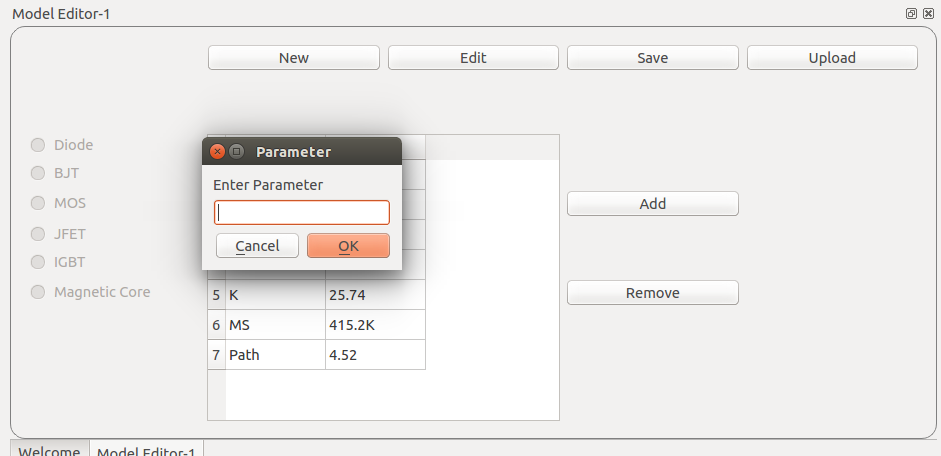
\includegraphics[width =\lgfig]{modeladd.png}
\caption{Adding the Parameter in a Library}
\label{modeladd}
\end{figure}

\begin{figure}
\centering
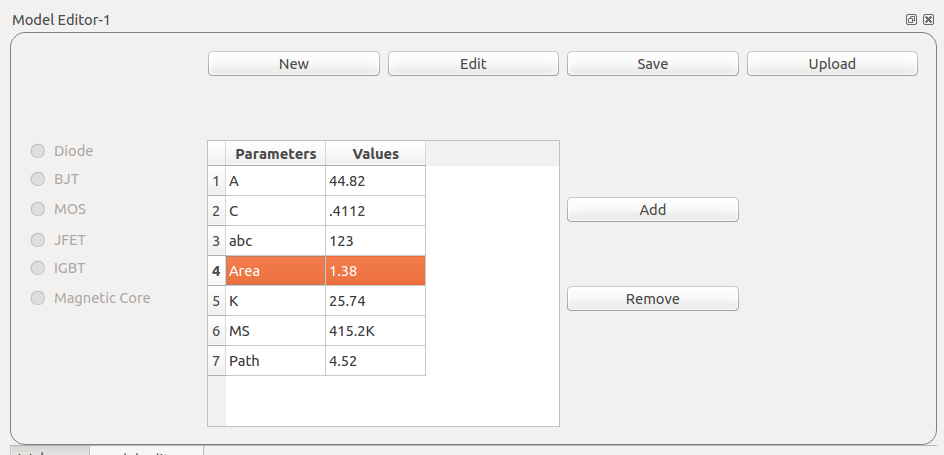
\includegraphics[width =\lgfig]{modelremove.png}
\caption{Removing a Parameter from a Library }
\label{modelremove}
\end{figure}

After the editing of the model library is done, the file can be saved by selecting the {\tt SAVE} button. These libraries are saved in the \textit{User Libraries} folder under \textit{deviceModelLibrary} directory.

\section{Editing Current Model Library}
The existing model library can be modified using {\tt EDIT} option. On clicking the {\tt EDIT} button the file dialog opens where all the library files are saved as shown in \figref{modeledit}. You can select the library you want to edit.
Once you are done with the editing, click on {\tt SAVE} button.

\begin{figure}
\centering
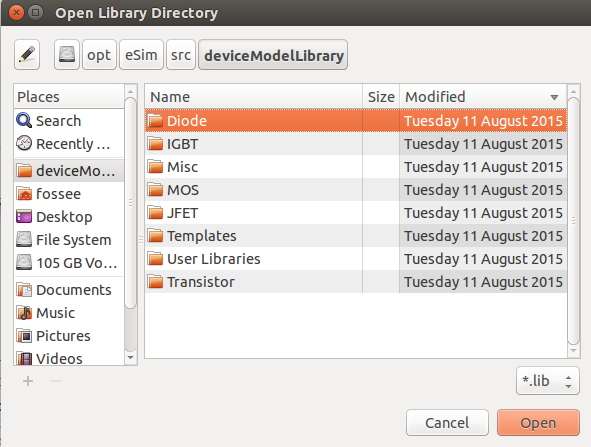
\includegraphics[width =\lgfig]{modeledit.png}
\caption{Editing Existing Model Library}
\label{modeledit}
\end{figure}

\section{Uploading external .lib file to eSim repository}
User can also upload external spice {\textbf{.model}} library files. These .model libraries can be downloaded online.  eSim directly cannot use the external .lib file. It has to be uploaded to eSim repository before using it in a circuit.
eSim provides the facility to upload library files using the {\textbf Upload} option in the {\textit 
{Model Editor}}. They are then converted into xml format, which can be easily modified from the eSim interface.
On clicking {\tt UPLOAD} button the library can be uploaded from any location. The model library will be saved with the name you have provided, in the \textit {User Libraries} folder of repository \textit{deviceModelLibrary}.
Example: You can download any model of Schottky diode from Spice website and save it as .lib extension on the system. Click on  {\tt UPLOAD} option and give the path. The lib file along with XML file is created in the {\tt eSim-2.0/library/deviceModeLibrary/UserLibraries if you are using v2.0 \linebreak and above versions \\
 eSim-1.1.3/src/deviceModeLibrary/UserLibraries if you are using \linebreak versions lower than 2.0 \\}. The uploaded library can be used for the existing part eSim\_Diode or the user can create a new model (part). Refer Chapter 8 on how to create a new part library model in eSim.
